The measurement of current $I$ was shown in Table \ref{tab-deg-0}.
\begin{table}[!h]
\begin{center}
\begin{tabular}{|c|c|c||c|c|c|}
\hline
\multicolumn{6}{|c|}{Rotation angle of 1/4-wave plate: $0^\circ$}\\
\hline
\multicolumn{6}{|c|}{Maximum Electric Current $I_0$ $4.785\pm0.001$ [$\mu A$]}\\
\hline
$\theta$&$I[\mu A]\pm0.01[\mu A]$&$I/I_0$&$\theta$&$I[\mu A]\pm0.01[\mu A]$&$I/I_0$\\
\hline
$0^\circ$	&	4.771	&	$0.997\pm0.0003$	&	$180^\circ$	&	4.781	&	$0.999\pm0.0003$	\\
\hline
$10^\circ$	&	4.651	&	$0.972\pm0.0003$	&	$190^\circ$	&	4.677	&	$0.977\pm0.0003$	\\
\hline
$20^\circ$	&	4.261	&	$0.890\pm0.0003$	&	$200^\circ$	&	4.300	&	$0.899\pm0.0003$	\\
\hline
$30^\circ$	&	3.660	&	$0.765\pm0.0003$	&	$210^\circ$	&	3.725	&	$0.778\pm0.0003$	\\
\hline
$40^\circ$	&	2.870	&	$0.600\pm0.0002$	&	$220^\circ$	&	2.955	&	$0.618\pm0.0002$	\\
\hline
$50^\circ$	&	2.053	&	$0.429\pm0.0002$	&	$230^\circ$	&	2.112	&	$0.441\pm0.0002$	\\
\hline
$60^\circ$	&	1.246	&	$0.260\pm0.0002$	&	$240^\circ$	&	1.300	&	$0.272\pm0.0002$	\\
\hline
$70^\circ$	&	0.617	&	$0.129\pm0.0002$	&	$250^\circ$	&	0.635	&	$0.133\pm0.0002$	\\
\hline
$80^\circ$	&	0.153	&	$0.032\pm0.0002$	&	$260^\circ$	&	0.179	&	$0.037\pm0.0002$	\\
\hline
$90^\circ$	&	0.001	&	$0.000\pm0.0002$	&	$270^\circ$	&	0.000	&	$0.000\pm0.0002$	\\
\hline
$100^\circ$	&	0.089	&	$0.019\pm0.0002$	&	$280^\circ$	&	0.103	&	$0.022\pm0.0002$	\\
\hline
$110^\circ$	&	0.468	&	$0.098\pm0.0002$	&	$290^\circ$	&	0.479	&	$0.100\pm0.0002$	\\
\hline
$120^\circ$	&	1.065	&	$0.223\pm0.0002$	&	$300^\circ$	&	1.094	&	$0.229\pm0.0002$	\\
\hline
$130^\circ$	&	1.820	&	$0.380\pm0.0002$	&	$310^\circ$	&	1.863	&	$0.389\pm0.0002$	\\
\hline
$140^\circ$	&	2.656	&	$0.555\pm0.0002$	&	$320^\circ$	&	2.737	&	$0.572\pm0.0002$	\\
\hline
$150^\circ$	&	3.475	&	$0.726\pm0.0003$	&	$330^\circ$	&	3.498	&	$0.731\pm0.0003$	\\
\hline
$160^\circ$	&	4.157	&	$0.869\pm0.0003$	&	$340^\circ$	&	4.159	&	$0.869\pm0.0003$	\\
\hline
$170^\circ$	&	4.601	&	$0.962\pm0.0003$	&	$350^\circ$	&	4.615	&	$0.964\pm0.0003$	\\
\hline
\end{tabular}
\caption{Measurement data for the 1/4-wave plate (rotation angle $0^\circ$).}\label{tab-deg-0}
\end{center}
\end{table}

The relation between rotation angle and light intensity was plotted in Figure \ref{fig-deg-0}.
\begin{figure}[H]
\centering
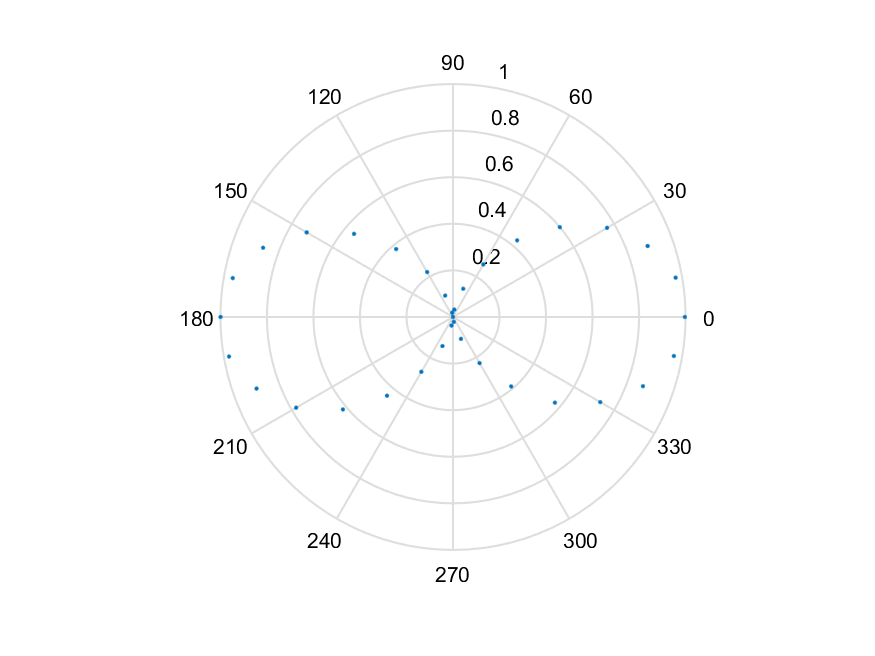
\includegraphics[scale=0.5]{deg-0.png}
\caption{$\theta$ vs. $I/I_0$ graph.}
\label{fig-deg-0}
\end{figure}
